\section{Ergebnisse}

\subsection{Vergleich Paramater}
\subsubsection{Taxi}

\subsubsection{Cliff}

\subsubsection{Frozen Lake}

\subsection{Vergleich Algorithmen}

Im folgenden werden die Ergebnisse beschrieben, welche bei dem Vergleichen der Algorithmen Q-Learning und SARSA entstanden sind.
Dabei wurde der Vergleich an den drei Reinforcement Learning Problemen Taxi, Cliff und Frozen Lake durchgeführt. Es wurden jeweils passende Paramater für das entsprechende Problem gewählt.
\subsubsection{Taxi}

\begin{figure}
    \centering
    \begin{subfigure}{.5\textwidth}
      \centering
      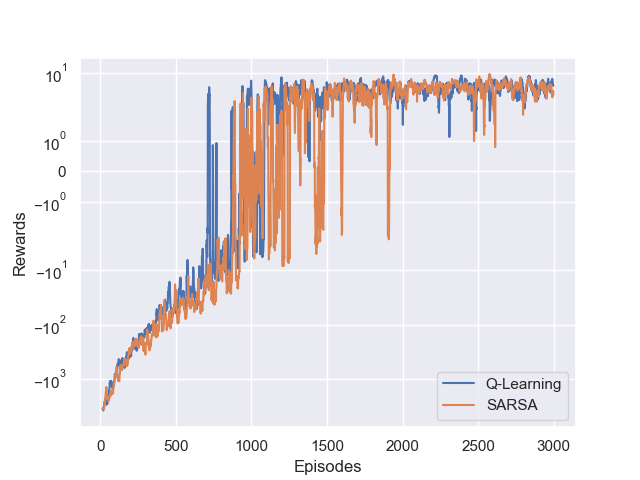
\includegraphics[width=1\linewidth]{taxi_q_vs_s_3000}
      \caption{Rewards}
      \label{fig:taxi_rew}
    \end{subfigure}%
    \begin{subfigure}{.5\textwidth}
      \centering
      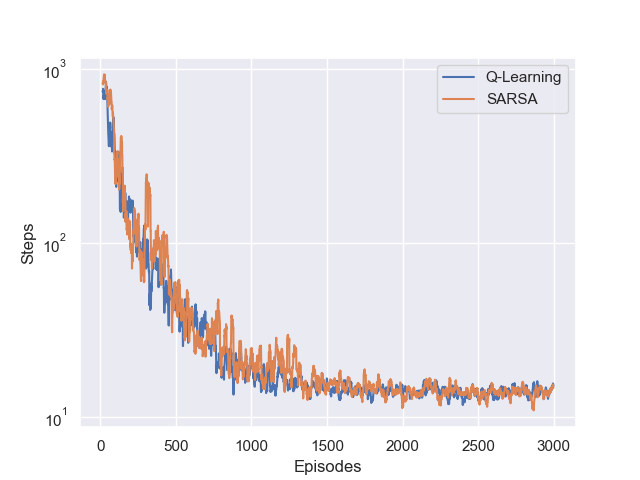
\includegraphics[width=1\linewidth]{taxi_q_vs_s_3000_steps}
      \caption{Steps}
      \label{fig:taxi_step}
    \end{subfigure}
    \caption{Taxi Problem over 3000 episodes during training}
    \label{fig:taxi_train}
\end{figure}

\subsubsection{Cliff}
\begin{figure}
    \centering
    \begin{subfigure}{.5\textwidth}
      \centering
      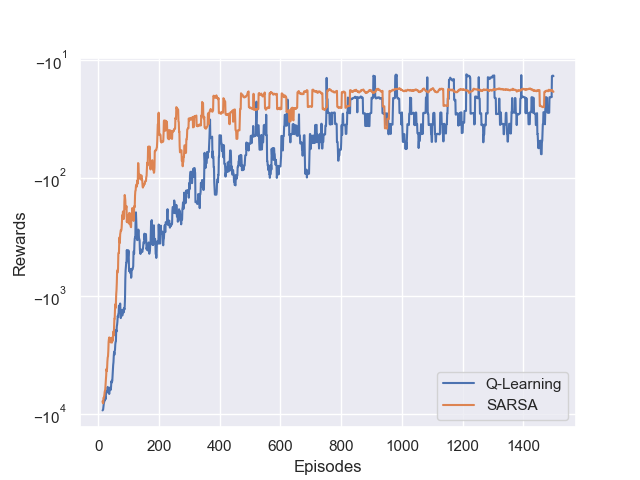
\includegraphics[width=1\linewidth]{cliff_q_vs_s_1500}
      \caption{Rewards}
      \label{fig:cliff_rew}
    \end{subfigure}%
    \begin{subfigure}{.5\textwidth}
      \centering
      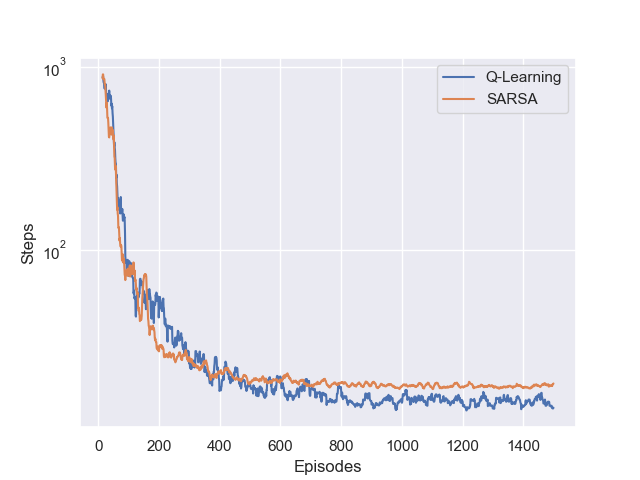
\includegraphics[width=1\linewidth]{cliff_q_vs_s_1500_steps}
      \caption{Steps}
      \label{fig:cliff_step}
    \end{subfigure}
    \caption{Cliff Problem over 1500 episodes during training}
    \label{fig:cliff_train}
\end{figure}

\begin{figure}
    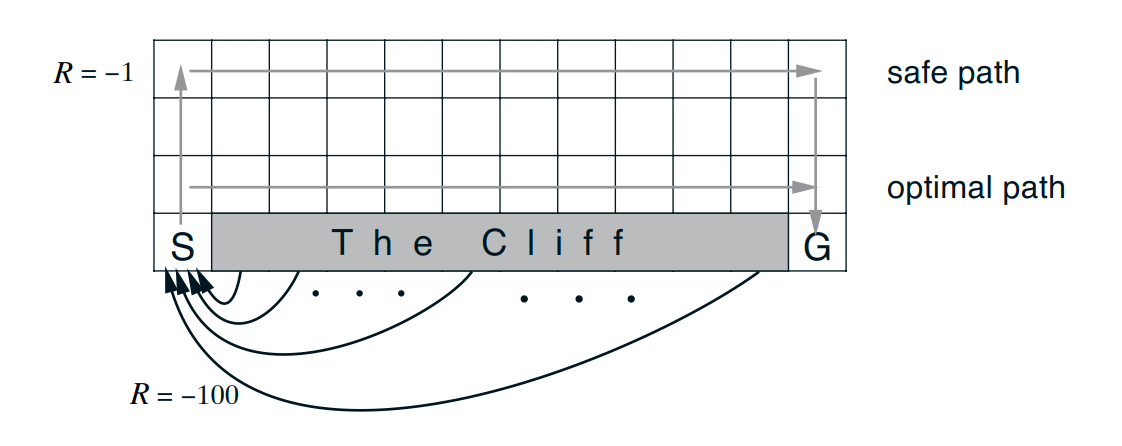
\includegraphics[scale=0.4]{cliff_path}
    \caption{Cliff Q-Learning vs SARSA Pfad}
    \label{fig:cliff_path}
\end{figure}

\subsubsection{Frozen Lake}

\begin{figure}
    \centering
    \begin{subfigure}{.5\textwidth}
      \centering
      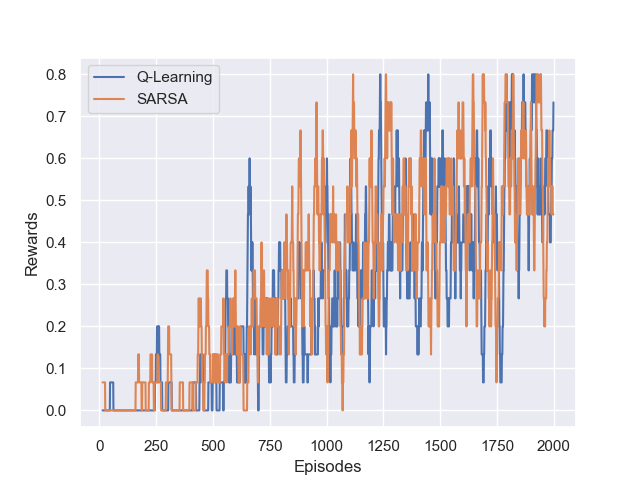
\includegraphics[width=1\linewidth]{frozen_lake_q_vs_s_2000}
      \caption{Rewards}
      \label{fig:frozen_rew}
    \end{subfigure}%
    \begin{subfigure}{.5\textwidth}
      \centering
      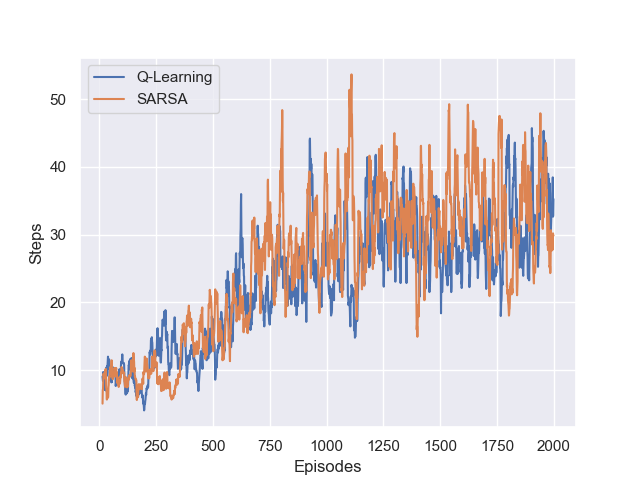
\includegraphics[width=1\linewidth]{frozen_lake_q_vs_s_2000_steps}
      \caption{Steps}
      \label{fig:frozen_step}
    \end{subfigure}
    \caption{Frozen Lake Problem over 2000 episodes during training}
    \label{fig:frozen_train}
\end{figure}

